% vim: set tw=0:
\documentclass{beamer}
\usepackage{graphicx}
\usepackage{hyperref}
\hypersetup{pdfborder={0 0 0 0}}

% Reasonable themes:
% Antibes Bergen Berkeley Berlin Frankfurt Goettingen Ilmenau Luebeck Malmoe
% Montpellier PaloAlto Rochester Singapore Szeged Warsaw bars boxes
% compatibility default lined plain shadow sidebar split tree
% And these ones include the author's name on every slide:
% Berkeley

% Declare themes.
\mode<presentation>
\usetheme{UWHEP}

% Personal macros.
\newcommand{\email}[1]{{\texttt #1}}
\newcommand{\newframe}[1]{\section{#1}
    \frametitle{\sc{#1}}}
\newcommand{\subframe}[1]{\subsection{#1}
    \frametitle{\sc{#1}}}
\newcommand{\supers}[1]{\ensuremath{^\textrm{#1}}}
\newcommand{\subs}[1]{\ensuremath{_\textrm{#1}}}
\newcommand{\ca}{\ensuremath{\sim}}
\renewcommand{\email}[1]{\href{mailto:#1}{\nolinkurl{#1}}}

% Author information.
\title{Storage at UW-Madison CMS Tier-2}
\author[Maier]{
    Will Maier \\ 
    {\tt wcmaier@hep.wisc.edu}}
\institute[Wisconsin]{University of Wisconsin - High Energy Physics}
\date[2010.09.22]{OSG Storage Forum, U. Chicago}
\logo{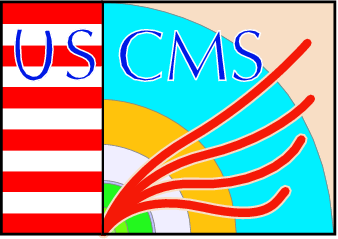
\includegraphics[height=0.6cm]{../../../Graphics/USCMS_logo.png}\hspace{.1cm}
\includegraphics[height=0.75cm]{../../../Graphics/UW_logo.png}}

\begin{document}

% http://indico.fnal.gov/conferenceTimeTable.py?confId=3377
% 15 min
% hardware/layout
% software
% monitoring/management
% evaluation
% plans

\begin{frame}
    \titlepage
\end{frame}

\section{Overview}
\begin{frame}
    \tableofcontents
\end{frame}

\section{Hardware}
\subsection{Summary}
\subsection{Core}
\begin{frame}
\begin{itemize}
	\item Four core dCache machines: PNFS, admin/misc, doors, hotspare
	\item 1 Gbps connections, SATA disks, 2x2 2.0 GHz Opterons, 16 GB RAM
	\item PNFS: RAID10 (10kRPM disks), 2x4 3.0 GHz Xeons
	\begin{itemize}
		\item Current configuration \ca{}12 months old
		\item Nearly saturated (again)\ldots{}need more IO
	\end{itemize}
	\item admin, doors, hotspare: commodity, nothing special
	\begin{itemize}
		\item No observed scaling issues with shared SRM/dcap door
	\end{itemize}
	% plot requests/time? files?
\end{itemize}
\end{frame}

\subsection{Cluster}
\begin{frame}
\begin{itemize}
	\item \ca{}50\% dedicated, \ca{}50\% shared with compute resources
	\item Dedicated nodes: mix of RAID6, RAID0 with 1 - 2 TB SATA disks
	\item Shared nodes: no RAID, .5 - 2 TB SATA disks (4 - 16 slots, 2 - 48 GB RAM)
	\item XXX pools on XXX nodes
	\item XXX Gbps network managed by campus
	% plot: TB/time
\end{itemize}
\end{frame}

\section{Software}
\subsection{Platform}
\begin{frame}
\begin{itemize}
	\item Scientific Linux 5.3/kickstart
	\item dCache v XXX
	\item SRM v XXX, gsiftp v XXX
	\item xrootd redirector thingy XXX
	% plot XXX
\end{itemize}
\end{frame}

\section{Management}
\subsection{Management} % cli, dcache_tools, dcache info provider
\begin{frame}
	\item 
\end{frame}

\subsection{Alerts} % nagios
\begin{frame}
\end{frame}

\subsection{Trends} % tsar
\begin{frame}
\end{frame}

\section{Evaluation}
\subsection{What Works}
\subsection{What Doesn't}

\section{Plans}

\section{Hardware}
\subsection{Summary}
\begin{frame}
\begin{itemize}
	\item \ca{}500TB of writable disk, 520 pools, 190 nodes
	\begin{itemize}
		\item Nodes host 2-4 pools each
	\end{itemize}
	\item Most of our network architecture is provided by campus, but we manage the switches
	\item We emphasize reliability and performance on central servers
	\begin{itemize}
		\item Reliability first: performance means nothing if the systems aren't up\ldots{}
		\item \ldots{}but work doesn't get done if clients are waiting to perform lookups on the central services
	\end{itemize}
	\item Make use of any and all available machines as cluster nodes
	\begin{itemize}
		\item Dedicated servers with large, local filesystems
		\item Batch nodes
		\item Retired test systems
	\end{itemize}
\end{itemize}
\end{frame}

\subsection{Network}
\begin{frame}
\begin{itemize}
	\item 10Gbps fiber uplink to campus, world
	\item 1Gbps Ethernet to all nodes and central servers
	\item Three stacks of Cisco 3750 switches
	\begin{itemize}
		\item Main stack bridged to others via 4Gbps Etherchannel
		\item Most connections use the stack backplanes; some node-to-node and node-to-WAN connections use the Etherchannels
	\end{itemize}
	\item \ca{}300 TB and 90 nodes on one side; \ca{}200 TB and 96 nodes on the other
\end{itemize}
\end{frame}

\subsection{Central Services}
\begin{frame}
\begin{itemize}
	\item Fast RAID for namespace database
	\begin{itemize}
		\item Need speed: database journals require lots of writes
		\item Need reliability: lots of pain if the database dies or becomes corrupted
		\item At Wisconsin: LSI RAID10 (4x250 GB 10k RPM SATA disks)
	\end{itemize}
	\item Databases and dCache daemons are happy to make use of available memory and cores
	\begin{itemize}
		\item At least 2GB/core; most servers have 16GB for 4 cores
	\end{itemize}
	\item All central servers on UPS; can survive short outages or shut down gracefully
	\begin{itemize}
		\item Filesystem corruption hurts
	\end{itemize}
	\item Otherwise, commodity hardware
	\begin{itemize}
		\item Fewer configuration profiles to manage
		\item Standard 7200 RPM SATA disks sufficient; no RAID (only namespace needs to persist)
	\end{itemize}
\end{itemize}
\end{frame}

\subsection{Cluster nodes}
\begin{frame}
\begin{itemize}
	\item Majority of storage on whitebox, dual-purpose batch and storage nodes
	\item Nodes stay in the cluster until it's too expensive to keep them running
	\begin{itemize}
		\item With five year warranties on disks, nodes can last a long time
		\item RAM upgrades or motherboard failures aren't worth the trouble if the node is out of warranty (standard three years)
	\end{itemize}
	\end{itemize}

	\begin{table}
	\begin{tabular}{rllll}
		\toprule
		Generation	& Disk (TB)	& RAM (GB)	& Cores	& Count	\\
		\midrule
	% main: g9, g10, s15, s5, opportunistic slots (45xg9x1TB, 24xg10x1.5TB, 10xs15x24TB, 9xs5x9TB)
		% 45 + 36 + 240 + 90 = 390TB
	% mr1: g7, g8 (27xg7x1TB, 5xg8x1TB)
		% 27 + 5 = 32 TB
	% mr2: g12, g14 (32xg12x3TB, 32xg14x4TB)
		% 96 + 128 = 224 TB
		1		& 1		& 2		& 2	& 32	\\ % g7,g8
		2		& 1-1.5		& 4-16		& 4	& 69	\\ % g9,g10
		3		& 3		& 16		& 8	& 32	\\ % g12
		4		& 4		& 16		& 8	& 32	\\ % g14
		\bottomrule
	\end{tabular}
	\caption{Wisconsin Dual-Purpose Cluster Nodes, 2005-2009}
	\label{cluster_nodes}
	\end{table}
\end{frame}

\begin{frame}
\begin{itemize}
	\item Dedicated storage
	\begin{itemize}
		\item Apple Xserve RAID with fiber channel to commodity controller node
		\item Whitebox with 24 local SATA disks, LSI RAID6
	\end{itemize}
	\begin{table}
	\begin{tabular}{rllll}
		\toprule
		Generation	& Disk (TB)	& RAM (GB)	& Cores	& Count	\\
		\midrule
		1		& 9		& 2		& 2	& 9	\\ % s5
		2		& 24		& 16		& 8	& 10	\\ % s15
		\bottomrule
	\end{tabular}
	\caption{Wisconsin Dedicated Storage Cluster Nodes, 2005-2009}
	\label{cluster_nodes}
	\end{table}
\end{itemize}
\end{frame}

\section{Software}
\subsection{Central Services}
\begin{frame}
\begin{itemize}
	\item Originally six central servers, with one service on each machine
	\item Now, dedicated nodes for PNFS, 'admin' services, SRM/dcap
	\item Hotspare system running and ready to cover for any of the above
	\item PNFS
	\begin{itemize}
		\item companion database
		\item PFM replication (for fast namespace lookups)
	\end{itemize}
	\item admin
	\begin{itemize}
		\item http monitor, admin interface, companion and billing databases
		\item Admin interface configured with SSH keys
		\item {\tt billingrep} live replicator (for access to the billing log)
	\end{itemize}
	\item SRM/dcap
	\begin{itemize}
		\item Only one door for each, and they live on the same machine
		\item Haven't observed performance problems
	\end{itemize}
	\item Hotspare
	\begin{itemize}
		\item {\tt /opt/d-cache} already present
		\item Ready for quick redeployment of a failed central service
	\end{itemize}
\end{itemize}
\end{frame}

\subsection{Cluster Nodes}
\begin{frame}
\begin{itemize}
	\item 30 GridFTP doors scattered across nodes
	\item Configure dCache JVMs so that 1.5GB RAM/core remains
	\begin{itemize}
		\item In most cases, four pool daemons, each with 400M JVMs
	\end{itemize}
	\item Most storage nodes also run Condor (one batch slot per core)
	\begin{itemize}
		\item Jobs are almost always running and fetching data
		\item dCache pushing files
		% \item (1000 slots x 2MB/s)/250 storage nodes
		\item No bottlenecks (yet) on the nodes, but the Etherchannels are troublesome
	\end{itemize}
\end{itemize}
\end{frame}

\section{Administration}
\subsection{Deployment}
\begin{frame}
\begin{itemize}
	\item {\tt /opt/d-cache} versioned by Mercurial, synced from AFS by CFEngine
	\begin{itemize}
		\item Clean upstream branch; local branch with changes
	\end{itemize}
	\item Configuration and installation automated by CFEngine
	\item CFEngine also installs extra RPMs, mounts PNFS, etc
	\item CFEngine handles upgrades, too:
	\begin{itemize}
		\item Merge new {\tt /opt/d-cache} with local
		\item Turn off services
		\item Push updates to all nodes and run {\tt install.sh} (CFEngine)
		\item Start services; revert to old {\tt /opt/d-cache} if necessary
		\item To roll back, revert to last known good {\tt /opt/d-cache} and server RPMs
	\end{itemize}
\end{itemize}
\end{frame}

\subsection{Replication}
\begin{frame}
\begin{itemize}
	\item Since we store data on commodity hardware (with no RAID), we make copies at the cluster level
	\item dCache's Replica Manager couldn't keep up with the flood of pool messages
	\item PFM performance slows with lots of pools and files
	\item {\tt billingrep} for low-latency, first order replication
	\begin{itemize}
		\item Watches billing log for file creations
		\item {\tt pp get file} to a random pool; replicated in seconds
		\item Not aware of pool cost/availability; doesn't recover if replicas disappear
		\item \url{http://code.hep.wisc.edu/dcache-tools}
	\end{itemize}
	\item {\tt pfm} for accurate policy enforcement
	\begin{itemize}
		\item Walks PNFS namespace (\ca{}10 minutes for 300k files), talks to each pool (20 minutes for \ca{}200 active pools)
		\item Finds available replicas for each file and adds or removes replicas depending on policy
		\item Policy defined by regular expressions matching logical file names
		\item At Wisconsin: No more or less than two replicas for each file
	\end{itemize}
\end{itemize}
\end{frame}

\subsection{Monitoring}
\begin{frame}
\begin{itemize}
	\item Nagios
	\item SAM, RSV
	\item root-owned files/directories
	\begin{itemize}
		\item {\tt find /pnfs/hep.wisc.edu/store/ /pnfs/hep.wisc.edu/osg/* -user root 2>/dev/null}
	\end{itemize}
	\item dCache Health Check
	\begin{itemize}
		\item Transfer from each GridFTP, dcap and SRM door
		\item Write new files into dCache; read them out and compare checksums
		\item Test transfers to and from FNAL via SRM
	\end{itemize}
	\item Stuck transfers
	\begin{itemize}
		\item Scan active transfers page for transfers with no significant activity
		\item Often indicates unavailable files or broken pools
	\end{itemize}
	\item Per-directory disk usage
	\begin{itemize}
		\item Walk PNFS and report disk usage (including replication) for the top directories
	\end{itemize}
	\item Absent pool report
\end{itemize}
\end{frame}

\section{Experiences}
\subsection{Usage}
\begin{frame}
\begin{itemize}
	\item Very few files lost (thanks to replication)
	\item Good performance in LoadTest
	\item Without fast disks on PNFS node, transfer pileups
	\item Merging lots of small files hurts
	\item Highly efficient analysis of large files (relatively small overhead)
\end{itemize}
\end{frame}

\subsection{Workflows}
\begin{frame}
\begin{itemize}
	\item Most local workflows involve extended analysis of large files or merging many small files
	\item Analysis:
	\begin{itemize}
		\item dCache works well without much modification
		\item Small tranfers overhead for small number of transfers, dcap provides fast access
		\item Relatively few outputs for each job
	\end{itemize}
	\item Merge:
	\begin{itemize}
		\item More common in SLHC workflows (and increasingly common in the future?)
		\item Most local approaches merge numerous small files in serial
		\item Unavailable files wait for timeout; during peak usage, time to fetch available files exceeds reasonable timeouts
		\item Improving PNFS performance helps, but this workflow is still inefficient on dCache
		\item Parallelizing merge process helps, too
	\end{itemize}
\end{itemize}
\end{frame}

\subsection{Plans}
\begin{frame}
\begin{itemize}
	\item Expand UPS coverage
	\item Local test stand/verify upgrades
	\item Add dcap doors
	\item Improve switch port efficiency so all nodes communicate across the same 16Gbps backplane
	\item Point {\tt billingrep} at database, not log
	\item {\tt pgpool} replication of PostgreSQL databases
	\item Centralize databases on high-performance server or provide faster disks on all central servers
\end{itemize}
\end{frame}

\end{document}
